\section{ParVSL}
I have forked the original VSL project into a new language which I named Parallel VSL, or ParVSL.
ParVSL is fully backwards compatible with VSL and will be compared against it for performance.

VSL was a good candidate for this project because it featured a complete, working Lisp implementation while being
small enough to be a manageable project. The entire VSL codebase consists of around 10000 lines of code, all of which
was originally contained within a single file. Before making changes in critical areas, I spent some time familiarising
myself with the code. This included splitting the project into multiple files, fixing a few obvious bugs, and porting
from C to C++.

\section{From C to C++}
The VSL language was written in the C programming language. C is a language with no standardised
multi-threaded model and no native support for multi-core programming. Furthermore, it has no well-defined
memory model, and no defined ordering of memory accesses. Multi-threaded programming
is only possible in C through a third-party library, such as \texttt{Windows threads} or the
the \texttt{POSIX threads} library on UNIX systems. Support has to be provided by individual compilers
and operating systems and can break between versions.

C++ is a superset of C and can compile existing, standard C code. The C++11 standard addresses the
above omissions, making C++ a multi-threaded language. While in some cases the implementation uses the same
libraries as the C equivalent (e.g. POSIX), I do not have to think about these details and the code
I write is fully portable. The only requirement is that a C++11 compliant compiler is used supporting
the target platform. As of today, the C++11 standard has matured enough
that all the large compiler vendors (i.e. GCC, Clang, Visual C++, Mingw, etc.) fully support it on the
major platforms (e.g. x86, ARM and SPARC).

The first change I have made to the implementation is to clear it of any incompatible code and compile it
with a C++ compiler. This mostly involved adding a few more explicit casts\footnote{e.g.
C++ is stricter than C about the need for \texttt{const} qualifiers on pointers that
may refer to C-style strings.}.
However, I also transitioned the code to idiomatic C++ as I analysed more parts of it
and became confident those changes wouldn't affect the semantics of the program.

\subsection{RAII classes}
\label{sec:raii}
The \emph{RAII (Resource Allocation Is Initialisation)} design pattern is common in C++ \cite[Item~37]{effective-cpp}.
It is a programming technique which binds the lifetime of resources to an object's lifetime. Normally,
C and C++ are manually managed, meaning all resources have to be carefully tracked by the programmer.
This makes it easy to introduce bugs when there is an attempted access to an unallocated resource,
or leaks when a resource is not released after use. C++ classes offer a solution to this problem.
Classes have both constructors and destructors, and these are automatically called when the object
is created and when it becomes unavailable (it goes out of scope or it is deleted), respectively.

We can use this mechanism to implement RAII. We simply make sure
the underlying resource is allocated in the constructor and deallocated in the destructor.
Smart pointers like \verb|std::unique_ptr| are a good showcase of the power of RAII. As soon as the
smart pointer objects become inaccessible (e.g. by going out of scope), the underlying pointer
is safely deleted, providing a primitive (but very effective) form of automatic reference counting.

When changing the codebase to use C++ features I found various opportunities to apply the RAII pattern:
for managing threads, shallow binding and for garbage collection synchronisation.

\section{Throughput vs latency}
When optimising for performance in a programming language, we have to analyse the trade-off between
total throughput and latency. Optimising for latency means minimising the duration of any individual
task in the program, and increasing availability. Optimising for throughput involves minimising the
total running time of the program.

In a CAS program the user is most likely to care about throughput, i.e. for computing the outputs of large
problem sizes as quickly as possible. The program is single-user and has a simple interface. The only case
for low latency is in the responsiveness of the graphical user interface. This is already provided by the
operating system so our main goal is directed towards maximising throughput in the application.
This is particularly important when designing the garbage collector.

\section{The read-eval-print loop}

The VSL Lisp system has a \emph{read-eval-print} loop at its core: it reads the next instruction, evaluates
it and prints the result. When evaluating performance, I carefully analysed the functions
called within this loop. These functions constitute the \emph{critical path}. The code on the critical
path is the most heavily used and should be as efficient as possible. When I modify it to enable
multi-threading, I pay special attention to not encumber it.

\section{Memory allocation}
Memory is managed by the interpreter. VSL allocates a large block of memory at the beginning,
which it then manages as a contiguous array. When running out of memory, an extra block of the
same size as the one in use is \verb|malloc|-ed, doubling the amount available. These blocks are
never freed until the end of the program. They are sorted by their pointer locations,
and behave as if they were \emph{joined} together to maintain the abstract model of contiguous memory.
Binary search is used to identify the block containing a location.

The allocations are efficient, using a simple pointer, called \emph{fringe} to indicate the start of the
free area of memory. An additional pointer \emph{limit} indicates the end of free memory. To allocate,
VSL checks whether there is enough space, then simply increments the fringe by the specified amount.
If the allocation would cross \verb|limit|, it triggers \emph{garbage collection}.

\begin{figure}[H]
    \centering
    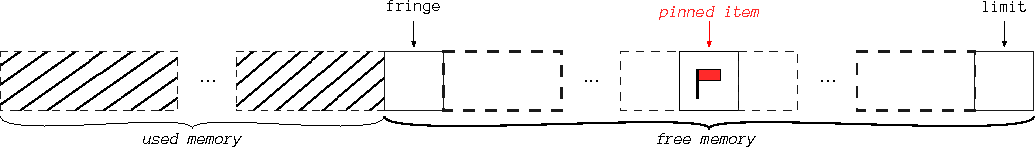
\includegraphics[width=1\linewidth]{vslalloc.pdf}
    \label{fig:vslalloc}
    \caption{Memory allocations in VSL}
\end{figure}

\section{Garbage collector}
An important feature of Lisp languages is the \emph{Garbage Collector} (GC). Garbage collectors allow the programmer
to design code without having to worry about the lifecycle of their data, the internal memory model or
managing pointers. This makes Lisp code significantly easier to write, leaving the burden of providing safety and
efficiency to the system.

In effect, the garbage collector is an important component of VSL and careful considerations
have to be made when modifying it. First of all, any bugs in the garbage collector may leave the memory in
an invalid state, corrupting the state of the program and leading to undefined behaviour in C. Such errors
are also very difficult to spot and debug, as they can go undetected until the particular region of memory
is accessed again.

\subsection{Cheney's algorithm}
The approach a garbage collector uses to deal with freed memory affects both its performance and memory usage.
Before the first garbage collection cycle, memory can simply be allocated in a continuous fashion, making it
compact and fast. When the garbage collector finds unreachable objects and eliminates them, they will leave
\emph{gaps} behind and cause \emph{fragmentation}.

The algorithm is \emph{stop-the-world}:
it requires pausing execution of the program until the entire collection is over.
The alternative, an \emph{incremental} GC would use minor collections which only partially reclaim memory.
Such an algorithm would only reduce latency at the expense of throughput and fragmentation.

Cheney's algorithm \cite{cheney} is a way of implementing a copying garbage collection.
The virtual \emph{heap} is divided into
two halves, and only one half is in use for allocations. The other half is considered free and used during garbage
collection. When the first half is full and garbage collection is triggered, all traceable objects are copied over
to the second half. Then, the two halves are swapped.

To start the tracing we need to consider a \emph{root set}: a subset of objects which are known to be in use.
One example of elements in the root set is the set of symbols that are in use at the start of garbage collection.
The stack also contains pointers to objects and must be scanned when computing the root set.
While these are the main components of the root set, the interpreter may contain others depending on language features
and implementation, all of which must be spotted and added.

Using the root set, we can trace all references to build the reachable set. Objects may contain references
to other objects, which are also considered reachable.
All objects in the reachable set must be kept during collection, while everything else may be safely collected.
Cheney's algorithm copies over the objects in the root set first. It also modifies their original location to become
a \emph{forwarding reference}: a note indicating that they were moved and what their new location is. Then, it scans
the newly allocated memory (the objects copied over) for more references.
For example, a list object will contain a reference to the rest of the list which is now also copied over.

Please refer to appendix \ref{sec:cheneycode} for a more detailed implementation of the algorithm.

\subsection{Conservative GC}

Garbage collection may start in the middle of a large computation and the references on the stack cannot be discarded.
One safe, but slow approach of dealing with this is to keep a virtual stack. Such a stack could be well typed and easily scanned to find
references. Another is to tag all data on the stack with an extra bit indicating which values are pointers. This approach
is used in OCaml \cite[Chapter~20]{rwoc}, yet it still has the disadvantage of limiting integer types and requiring an extra
instruction (i.e. shift) during runtime.

Instead, VSL uses a \emph{conservative} GC, meaning it over-approximates the root set.
It treats all values on the stack as potential references, called \emph{ambiguous} roots.
This means we are overestimating the set of roots. Unlike \emph{unambiguous} roots (like the symbol table above), we
have to be careful when handling these values, and cannot manipulate them as ordinary Lisp objects, which rules out
copying them over. The solution was
to \emph{pin} them, i.e. mark them in the heap so they are not moved. Listing \ref{code:scanpinned}
shows the process of pinning objects.
Any location on our heap which is pointed to by an ambiguous root is pinned and not copied over.
Additionally, the \texttt{allocate} function will have to check for pinned items on the heap and skip over them.
When building the entirety of REDUCE, the number of pinned items does not reach 300.
Considering memory used is in the order of megabytes, these pinned locations cause negligible fragmentation.

\begin{code}
\begin{minted}[breaklines,mathescape]{c++}
int main() {
  ...
  // before starting the Lisp interpreter
  c_stack_base = approximate_stack_pointer();
  ...
}

void garbage_collection() {
  c_stack_head = approximate_stack_pointer();

  // scan the stack from its head to base
  for (uintptr_t s  = c_stack_head;
                 s  < c_stack_base;
                 s  += sizeof(LispObject))
    if (in_heap(s)) { // check if s points to the virtual heap
      set_pinned(s); // found an ambiguous root
    }
  ...
}
\end{minted}
\caption{Scanning the stack before GC for ambiguous references.}
\label{code:scanpinned}
\end{code}

\subsection{Running single-threaded}

I decided to run the garbage collector on a single thread. This approach still requires synchronisation with all running
threads, however it requires no extra inter-locking during collection. Implementing a safe multi-threaded garbage collector
efficiently would probably merit its own project. I believe that for the small hardware thread counts of current day computers
a single threaded algorithm is adequate, not having to deal with data races and inter-locks. However, his may change as
CPU core counts increase.

\section{Symbols and variable lifetime}
As the original language is decades old, its mechanism for variable lifecycle is not in line with that of modern languages.
This mechanism was counter-intuitive at first, and is lacking in providing safety to the user of the language.

There are two lifetime specifiers for \emph{symbols}: \emph{global} and \emph{fluid}. It is important to note that they
do not refer semantically to variables but only to symbol names.

A \emph{global} symbol has only a single globally visible value. That means you cannot bind the name to any local
variable. For instance if \texttt{x} is declared global, it then cannot be used as a function parameter name, or in a
let binding.

A \emph{fluid} variable has a global value, but can also be locally bound. Fluids behave more like globals do
in other languages, allowing the name to be reused.

\texttt{Let} bindings and function parameters introduce \emph{local} symbols. If the symbol name is already declared global,
it will result in an error. If it is a fluid and has a global value, that value will be shadowed for the lifetime
of the binding.

\section{Debugging tools}

Debugging multi-threaded code is especially difficult and I
needed the right tools to help me find the source of issues. I used
the \verb|gdb| \cite{gdb} debugger to step through code and find the source
of the problem. I used \verb|gprof| \cite{gprof} to profile my code and find
the areas on the critical path which needed optimisations the most. Finally,
I used \verb|valgrind| \cite{valgrind} to analyse ParVSL for memory
problems, data races and undefined behaviour.
